\section{Development View}
\label{sec_development}

\subsection{Overview}

This view describes the architecture that supports the software development process and is of interest to those stakehoolders involved in building, testing, maintaining and enhancing the software. This section will detail the software layers and the boundaries that exist between them.

\subsection{Stakeholders}

\textbf{\textit{Developers, Maintainers, Researchers, Testers, Users}}

\textit{A description of all stakeholders is contained in Section \ref{sec:stakeholders}.}


\subsection{Layers}

The various software layers are shown in Figure \ref{fig:safecrypto_components}. In this diagram the software scheme has an interface with the Interface Layer of the library that allows an arbitrary scheme that adheres to the \textit{Schemes} interface to be used. Each scheme can implement an interface to a variety of hashes, NTT's, CSPRNGs, entropy coders, etc. in the Utility Layer. This permits the source code in the Schemes Layer to remain generic, while platform and application specific source code can be implemented within the Utility Layer. For example, arithmetic, hash and CSPRNG functions that are optimised for a specific embedded processor can be assigned dynamically when an instance of the library is instantiated.

\begin{figure}[!h]
\centering
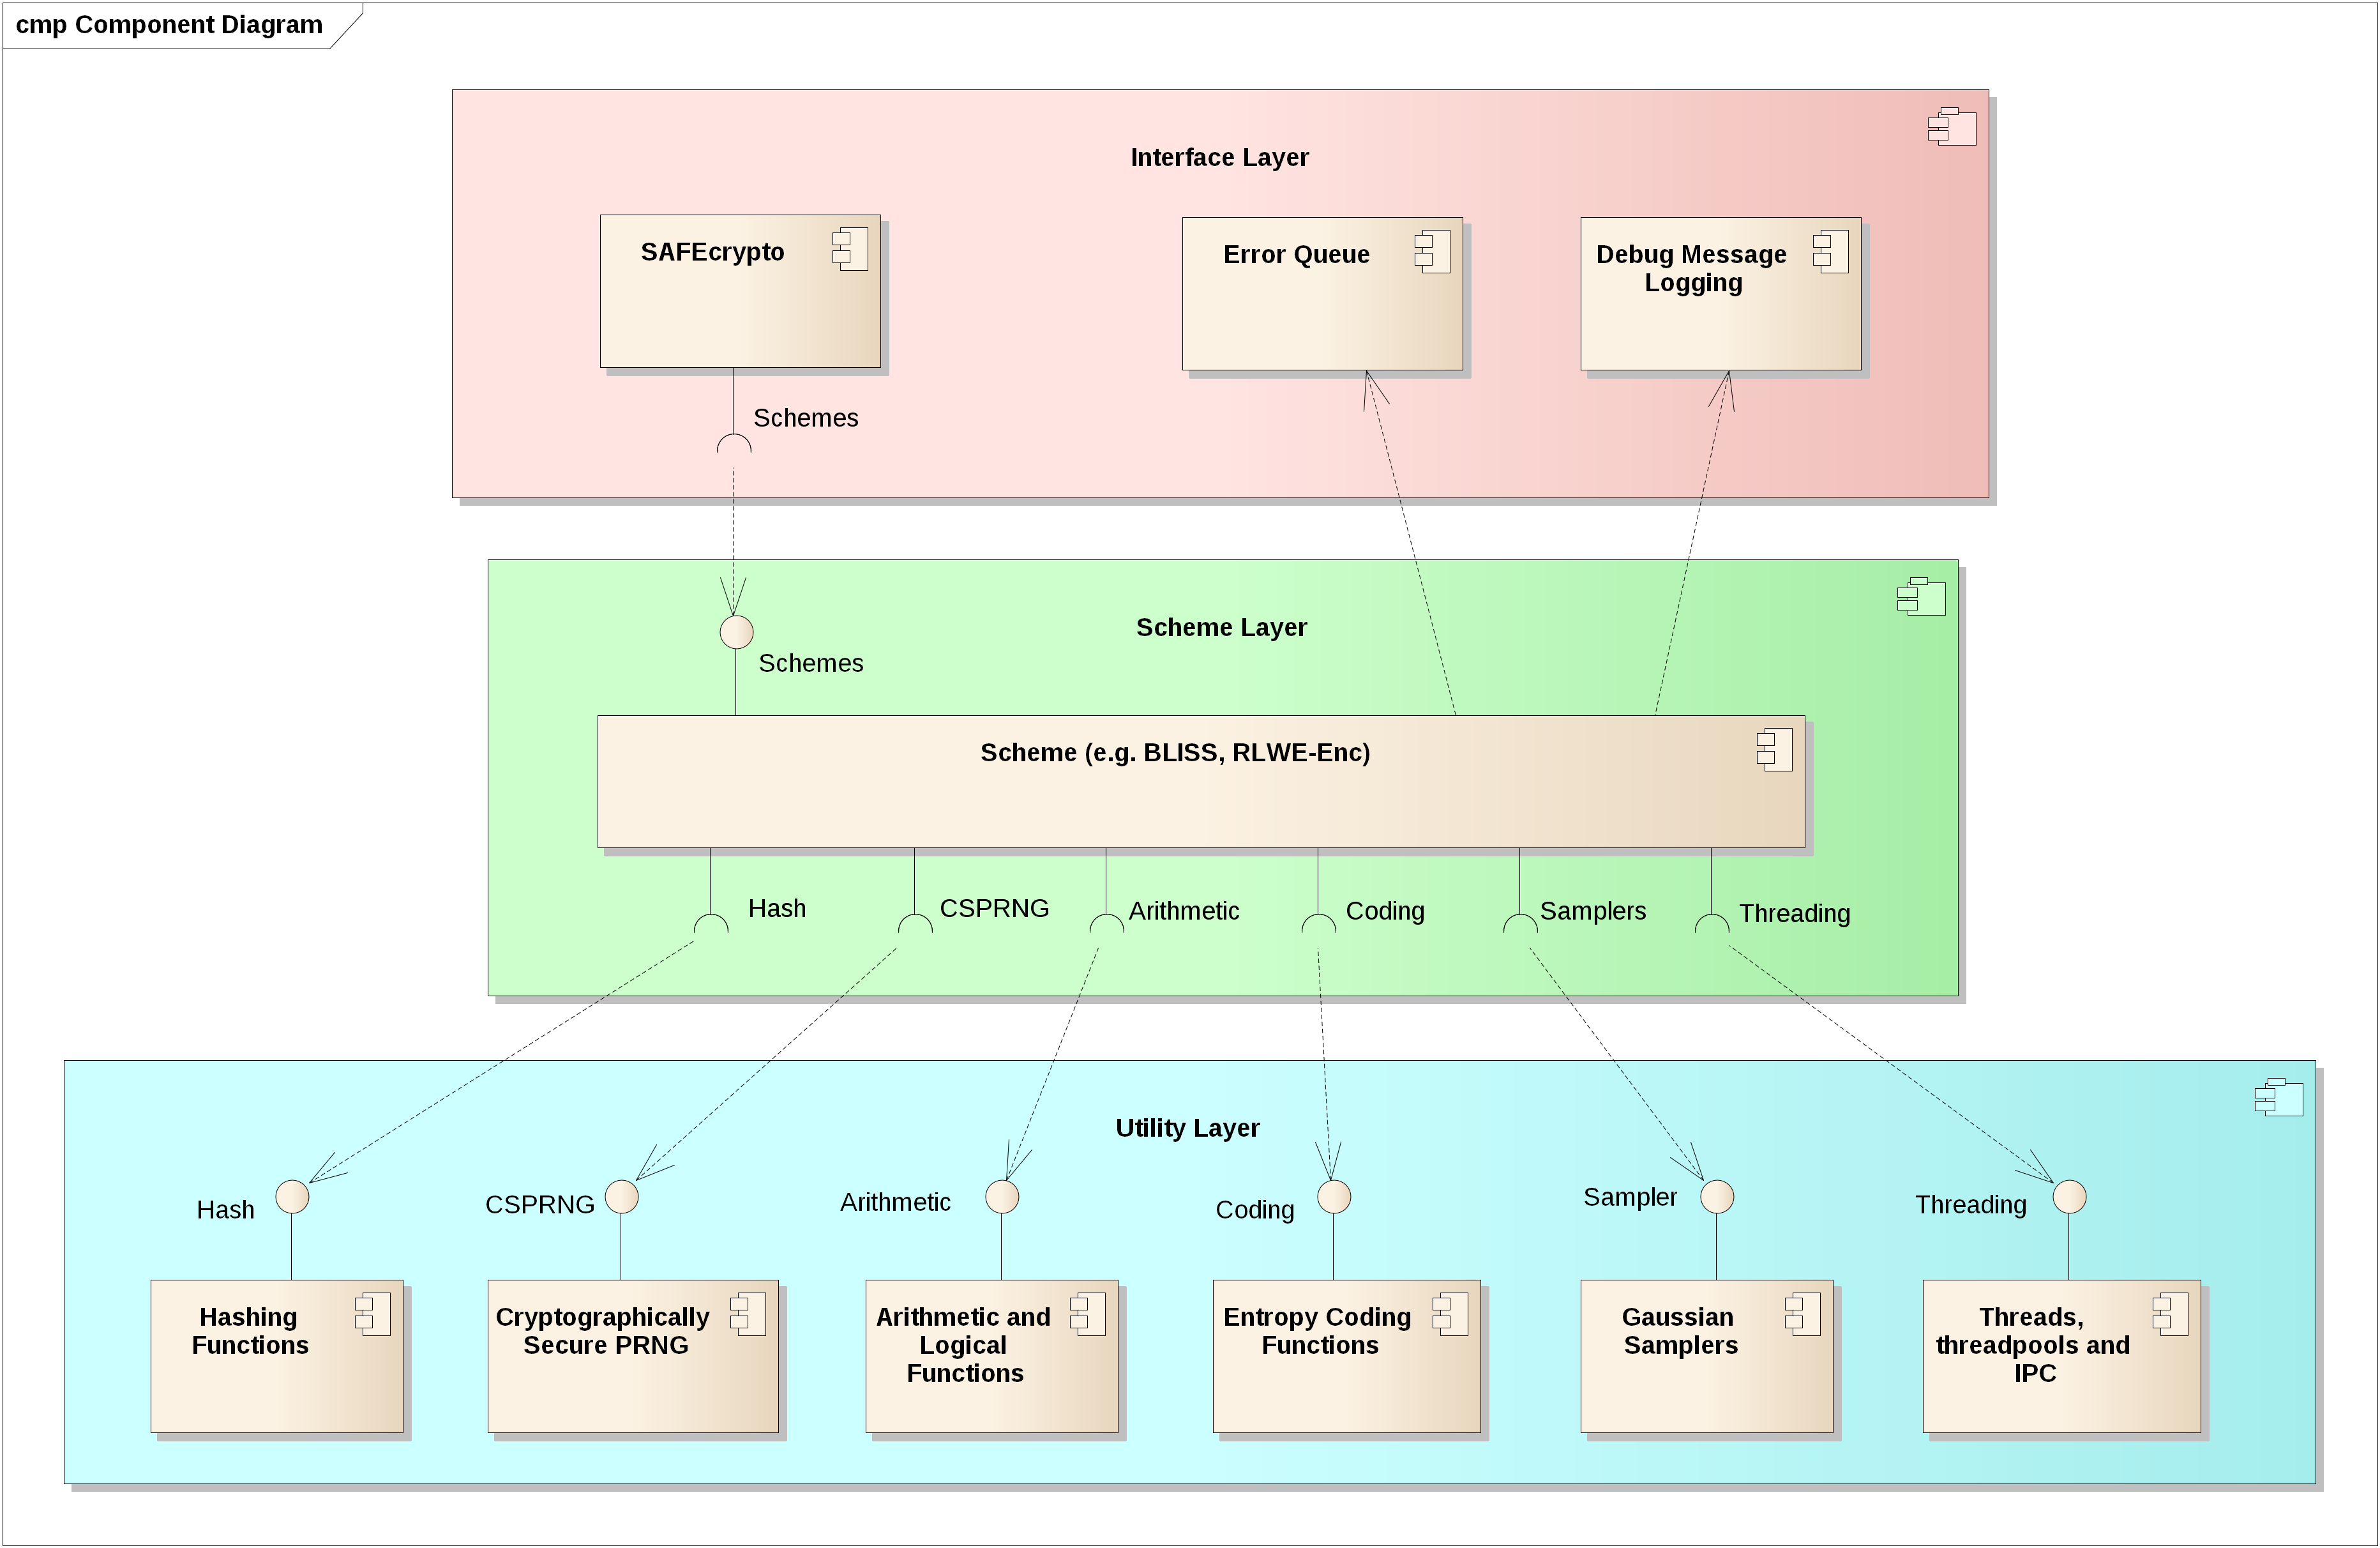
\includegraphics[width=\textwidth]{libsafecrypto_development_view.png}
\caption{Component diagram of SAFEcrypto library}
\label{fig:safecrypto_components}
\end{figure}

\subsubsection{Interface Layer}

The Interface layer contains all of the components needed to allow interaction with an end-user. It encompasses the external API and the top-level of the software that acts as a glue for all underlying software layers. It is responsible for selecting the relevant function pointers for the selected scheme and maintaining the error and debug interfaces.

\subsubsection{Scheme Layer}

The Scheme layer contains the components used to provide the lattice-based cryptographic schemes within the software. These schemes are implemented as high level source code that adheres to a predefined internal API to enable them to be easily mapped to the interface. The schemes are entirely reliant on the Utility Layer to provide all mathematical, cryptographic and multi-threading functionality.

\subsubsection{Utility Layer}

The Utility layer contains all components that act to support the Scheme layer by providing basic components for arithmetic, random number generation, hashing functions etc. It is intended that the Utility Layer will be self-contained and will not be reliant on external third-party libraries. This will provide the added benefit of providing a common platform on which to evaluate various Lattice-based cryptographic schemes in a fair manner. It is envisaged that this Utility Layer will provide both generic and optimised versions of various routines, that are both run-time and compile-time selectable.


